\label{c:Experiments}
The experiments chapter first describes the final experimental pipeline, which is divided into the stereo camera calibration (\autoref{sec:Calibration}) and into the actual reconstruction (\autoref{sec:Reconstruction}) and secondly follows several experimental sessions to point out problems and results which occurred during the tests.

\section{Stereo Camera Calibration}\label{sec:Calibration}
The stereo camera calibration estimates the intrinsic and extrinsic parameters of a set-up of two uncalibrated cameras. The calibration is divided into first capturing image pairs of the checkerboard pattern (\autoref{ssec:PatternSequence}) and then estimating the parameters in the \textit{Stereo Camera Calibrator Toolboox}\index{Stereo Camera Calibrator Toolbox} in MATLAB (\autoref{ssec:estimateStereoParams}). The camera set-up used in the camera calibration must not be changed at all for the rest of the session: the sequence recorded for the actual 3-D reconstruction needs to have the same parameters.    

\subsection{Capturing Sequence of Calibration Pattern in TimeBench}\label{ssec:PatternSequence}
The two cameras should be set-up next to each other with little to no rotation. For stereo display (anaglyphic display) the cameras need to be placed about 55 mm apart, which is about the distance between our eyes. Since this thesis does not create stereoscopic displays, the cameras' baseline is set to approximately 19 cm, which is the minimum distance the two cameras can be apart from each other due to the camera bodies.\footnote{Cameras which are placed farther apart from each other resolve in greater reconstruction accuracy.} (\cite{StereoCalib.2016}).  

TimeBench should be only started after the two high-speed cameras have already been connected to the computer, otherwise the cameras may not be recognized by the software. After the hardware was installed (see \autoref{sec:architecture} for the cable set-up), the two cameras need to be dragged into a \textit{synchronization group} and the following configurations are recommended (\autoref{fig:timebanchRecord} shows a screenshot of the connected and synchronized cameras in Timebench): 

\begin{enumerate}[i]
\item Both cameras: set the frame rate to 70 fps\footnote{The smaller frame rate gives more time for positioning the calibration pattern in different angles, since the data amount is decreased to the lower frame rate.}
\item Right camera: check the box \enquote{Is Master} to set the right camera as the synchronization master.
\item Both cameras: set the exposure time slightly shorter than 1/frame rate.
\item Right camera: do not forget to white balance 
\end{enumerate}

\begin{figure}[htbp]
		\centering
		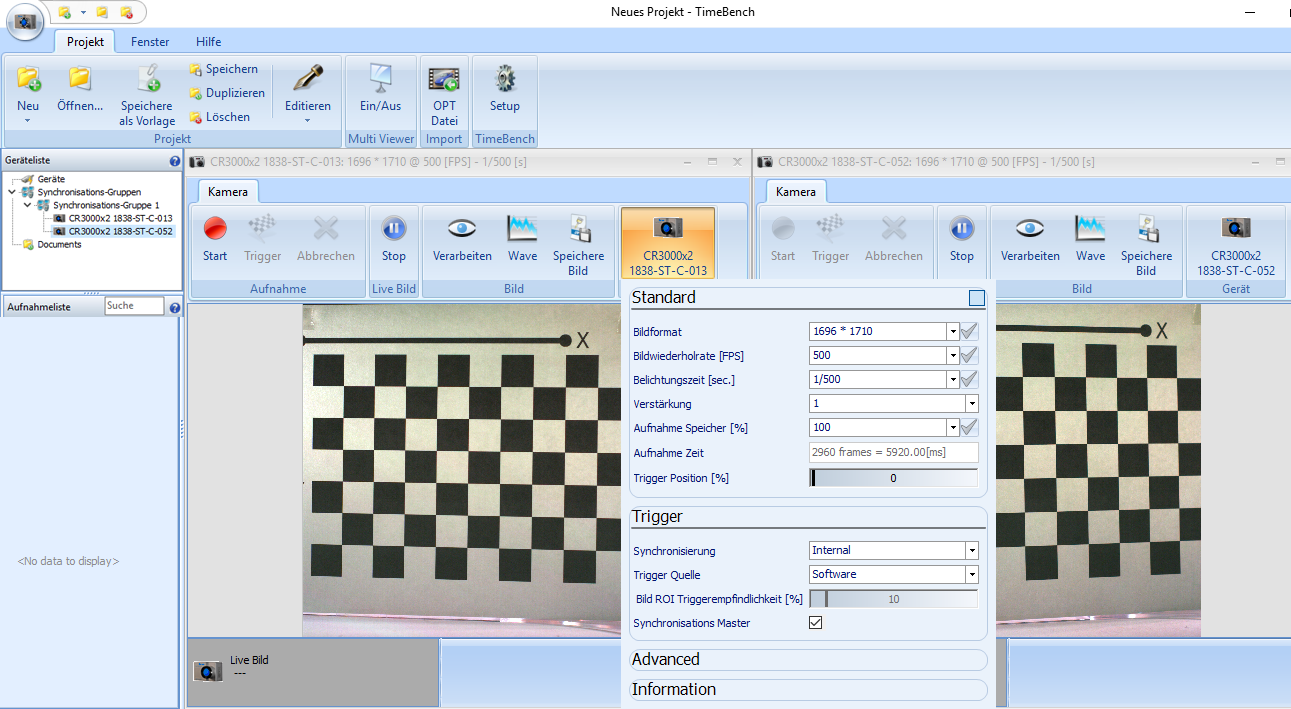
\includegraphics[width=1.0\textwidth]{figures/timebenchRecord}
		\caption[The views of two synchronized cameras and their capturing options in TimeBench]{The views of two synchronized cameras and their capturing options in TimeBench (\textit{source: software TimeBench owned by} \cite{Optronis.2016}).}
		\label{fig:timebanchRecord}
\end{figure}

Once the cameras are synchronized and configured the capturing of the calibration pattern images can begin. The pattern should be hold roughly at the same distance the objects will be placed in the actual scene. It needs to be in focus and must be fully visible in the view of both cameras. After starting the capturing sequence by clicking \enquote{Start} in the software and also activating the external trigger, the checkerboard pattern needs to be moved in different angles till the sequence stops. Out of the recorded image sequence 10-20 different image pairs have to be chosen (\autoref{fig:timebenchSequence} shows the timeline with the captured images of a session). Extreme angles are not likely to be detected later in MATLAB. 

\subsection{Estimating Stereo Parameters in Matlab}\label{ssec:estimateStereoParams}

(\cite{StereoCalib.2016})
problems with high speed cams vs. normal cams!
\begin{itemize}
\item brauch sehr viel Zeit
\item Beleuchtung
\item zusammenspiel software hardware
\item rectification problem (see urls below)
\end{itemize}



\todo{Problem with rectification:}
\url{http://www.mathworks.com/matlabcentral/answers/231808-problem-with-rectify-stereoimages}
-> not solved

\url{http://www.mathworks.com/matlabcentral/answers/247432-stereo-calibration-wrong-output-size-of-image}

\url{http://www.mathworks.com/matlabcentral/answers/155806-does-the-stereo-calibration-tutorial-work-for-angled-cameras}

\url{http://www.mathworks.com/matlabcentral/answers/231808-problem-with-rectify-stereoimages}

\url{http://www.mathworks.com/matlabcentral/answers/259267-camera-calibration-camerapose-vs-extrinsic}